\documentclass[a4paper,10pt,oneside]{scrartcl}
\usepackage[utf8x]{inputenc}
\usepackage[T1]{fontenc}
\usepackage[ngerman]{babel}
\usepackage[bookmarks=false,pagebackref,bookmarksnumbered]{hyperref}
\usepackage{pgf}
\usepackage{tikz}
\usetikzlibrary{arrows,automata}
\usepackage{multirow}
\usepackage[german]{fancyref}
\usepackage{float}
\usepackage{wrapfig}
\hyphenation{Ver-bund-wahr-schein-lich-keits-ver-tei-lung}

\usepackage[hscale=0.9,vscale=0.9]{geometry}

%opening
\title{Vergleich Probabilistischer Graphischer Modelle}
\author{Bernhard Häussner}

\begin{document}

\section*{Vergleich Probabilistischer Graphischer Modelle}

\textit{Vortrag zum Seminar Ausgewählte Themen des Web 2.0, von Bernhard Häussner am 18. Juni 2013.  }\\

Probabilistische graphische Modelle (PGMs)\cite{koller2009probabilistic} werden im Rahmen künstlicher Intelligenz interdisziplinär angewendet. Sie finden sich heute Anwendung im Rahmen des Web 2.0. Hierdurch werden neue Datenquellen verarbeitet, etwa Profildaten in sozialen Netzwerken. Sie stellen Verbundwahrscheinlichkeitsverteilungen $P(X_1,X_2,\dots,X_n)$ über "`viele"' Zufallsvariablen dar. Sie können von Computern auf maschinenlesbaren Daten deterministisch, objektiv und schnell angewendet werden.

\begin{minipage}{0.25\textwidth}
\centering
\begin{figure}[H]
\caption{\label{fig:pdgforest}Beispiel für den Abhängigkeiten-Wald eines probabilistischen Entscheidungsgraphen}
\begin{tikzpicture}
  %[->,>=stealth',shorten >=1pt,auto=left,every node/.style={circle,draw}]
  [scale=0.9,->,>=stealth',shorten >=1pt,auto=left,every node/.style={circle,draw}]
  \node (nf) at (1,3) {Farbe};
  \node (nm) at (3,2)  {Muster};
  \node (ng) at (1,1)  {Gift};

  \path (nf) edge (nm);
  \path (nm) edge (ng);

\end{tikzpicture}
\end{figure}
\end{minipage}\hfill
\begin{minipage}{0.65\textwidth}
\centering
\begin{figure}[H]
  \caption{\label{fig:datagraphs}Size/Likelihood-Kurven mit empirischen Daten aus \cite{nielsen2006empirical}}
  \centering
  %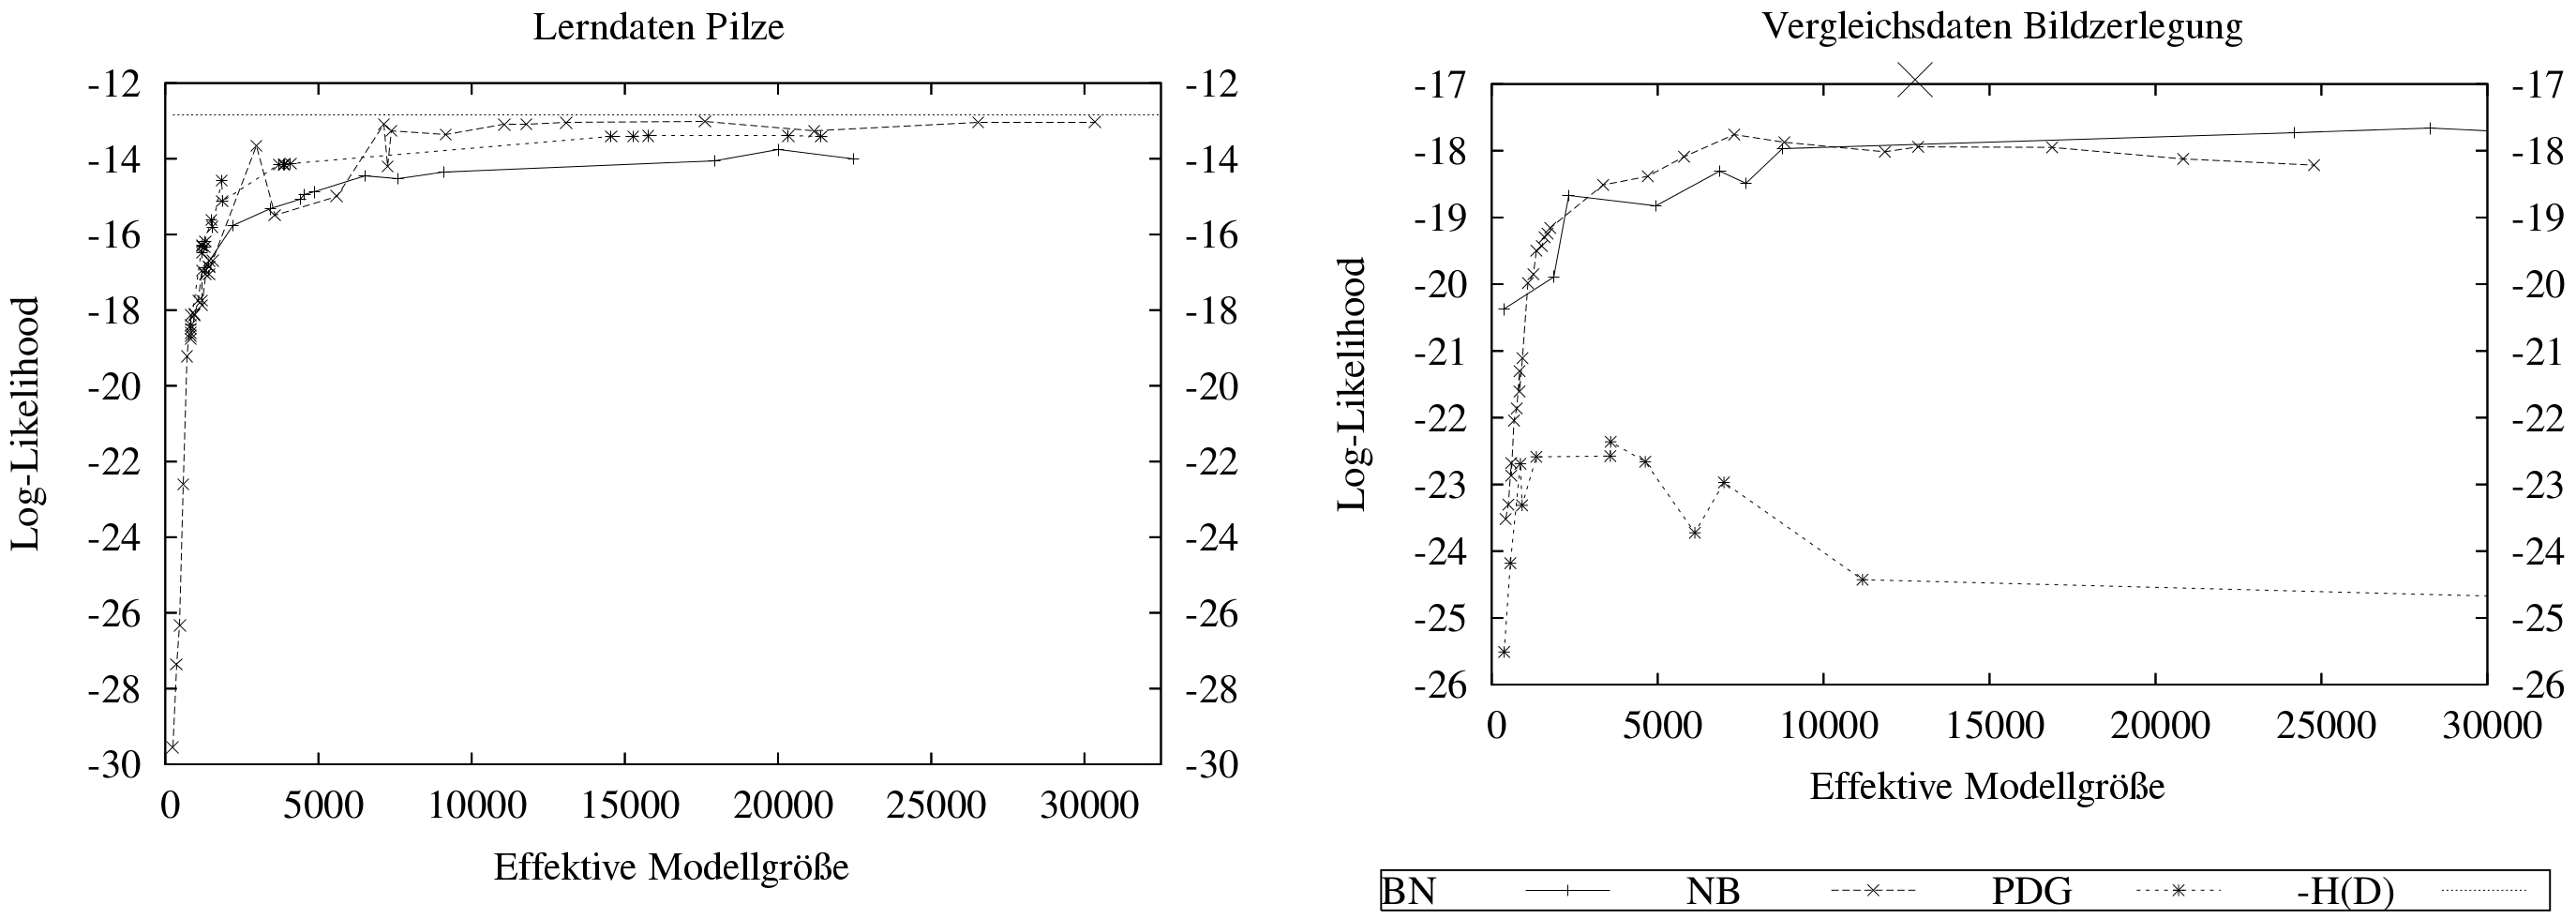
\includegraphics[width=0.7\textwidth]{graphs.png}
  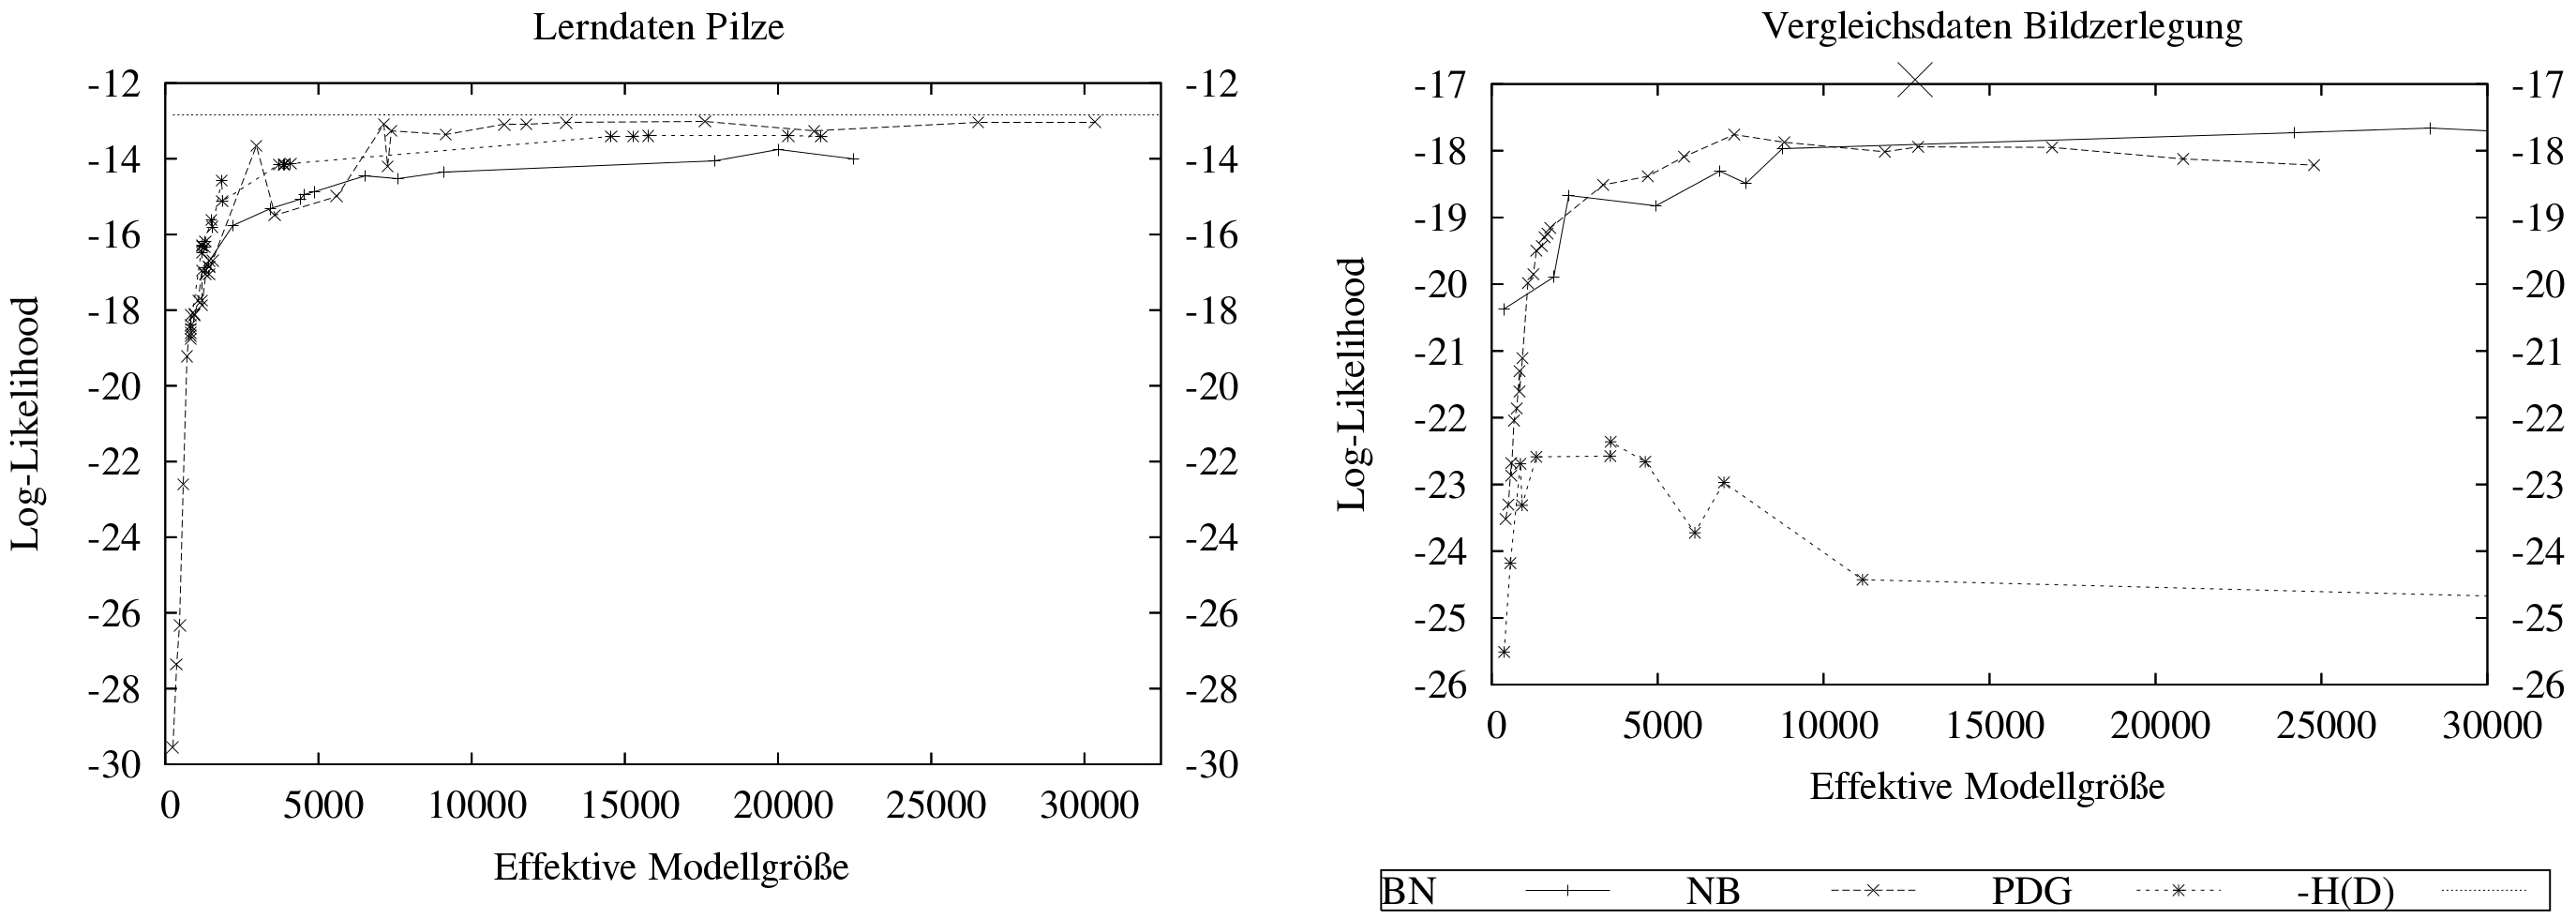
\includegraphics{graphs.png}
\end{figure}
\end{minipage}


\subsection*{Naive Bayes-Modelle}

Bei naiven Bayes-Modellen (NB) konstruiert man eine unbeobachtbare Zufallsvariable $C$. Die Zustände von $C$ nennt man Klasse oder Komponente. 
Es wird angenommen, dass in Abhängigkeit von $C$ alle Zufallsvariablen unabhängig sind. Somit entsprechen sie einem einfachen bayesschen Netz mit $C$ als Wurzel und den Zufallsvariablen als Blättern. Für die bedingten Unabhängigkeiten ergibt sich für je zwei Zufallsvariablen $(X_i \perp X_k | C)$. 

\subsection*{Probabilistische Entscheidungsgraphen}

Probabilistische Entscheidungsgraphen (engl. probabilistic decision graphs, PDG) nach \cite{bozga1999representation} drücken, anders als in bayesschen Netzen, Wahrscheinlichkeitsverteilungen in Abhängigkeit von bestimmten Variablenbelegungen aus.

Sie bestehen aus zwei kaskadierenden Graphen, zum einen aus einem Wald mit Knoten für die Zufallsvariablen und Abhängigkeiten zwischen diesen, zum anderen aus gewurzelten gerichteten azyklischen Graphen mit Knotenmengen für jede Zufallsvariable. Für jeden möglichen Wert der Zufallsvariable gibt es genau eine Kante zu einem Nachfolger-Knoten. Jeder Knoten wird annotiert mit einer Wahrscheinlichkeitsverteilung. Für jede Variablenbelegung wird jeweils ein Knoten erreicht, indem man den Kanten wie bei einem herkömmlichen Entscheidungsbaum folgt. Für die Verbundwahrscheinlichkeitsverteilung ergibt sich dann in Abhängigkeit der Wahrscheinlichkeitsverteilungen $P_{i,k}$ der durch Variablenbelegung erreichten Knoten:  $P(x_1,x_2,\dots,x_n) = \prod_{i=1}^n P_{i,k}(x_i) $. Für ein Beispiel zum Thema Pilze, siehe \fref{fig:pdgforest}.



\subsection*{Vergleich}

Bei \cite{nielsen2006empirical} werden die zwei Methoden und bayessche Netze verglichen, indem automatisch gelernte Modelle in Genauigkeit, Effizienz und Geschwindigkeit gemessen werden. Die Ergebnisse wurden wie in \fref{fig:datagraphs} graphisch aufbereitet. Der erwartete Geschwindigkeitsvorteil von NB gegenüber BN durch die einfachere Netzstruktur konnte hier experimentell nicht bestätigt werden. Über die Gesamtheit der Graphen erkennt man, dass BN bei keinem Datensatz sehr schlechte Ergebnisse zeigte. 

Keine Methode steht generell hinter den anderen zurück. Naive Bayes-Modelle und probabilistische Entscheidungsgraphen lassen sich leichter implementieren und weisen oft dennoch vergleichbare Qualitäts- und Geschwindigkeits-Charakteristika wie bayessche Netze auf. Bayessche Netze konnten jedoch unabhängig von der Beschaffenheit der Daten stets akzeptable Modelle bilden. Somit empfiehlt sich eine gleichberechtigten Anwendung der drei Methoden im Bereich des Web 2.0. 

\bibliography {haeussner}
\bibliographystyle{splncs}
\end{document}
